\documentclass{article}
\usepackage[utf8]{inputenc}
\usepackage{graphicx}
\usepackage{hyperref}
\usepackage{float}

\title{PSE Offline Meetings}
\author{PSE Project Team}
\date{\today}

\begin{document}

\maketitle

\section*{Overview}

This document contains images, notes, and documentation from offline meetings related to the PSE project.

\section*{First Meeting (Saturday, 19th April 2025)}

\begin{figure}[H]
    \centering
    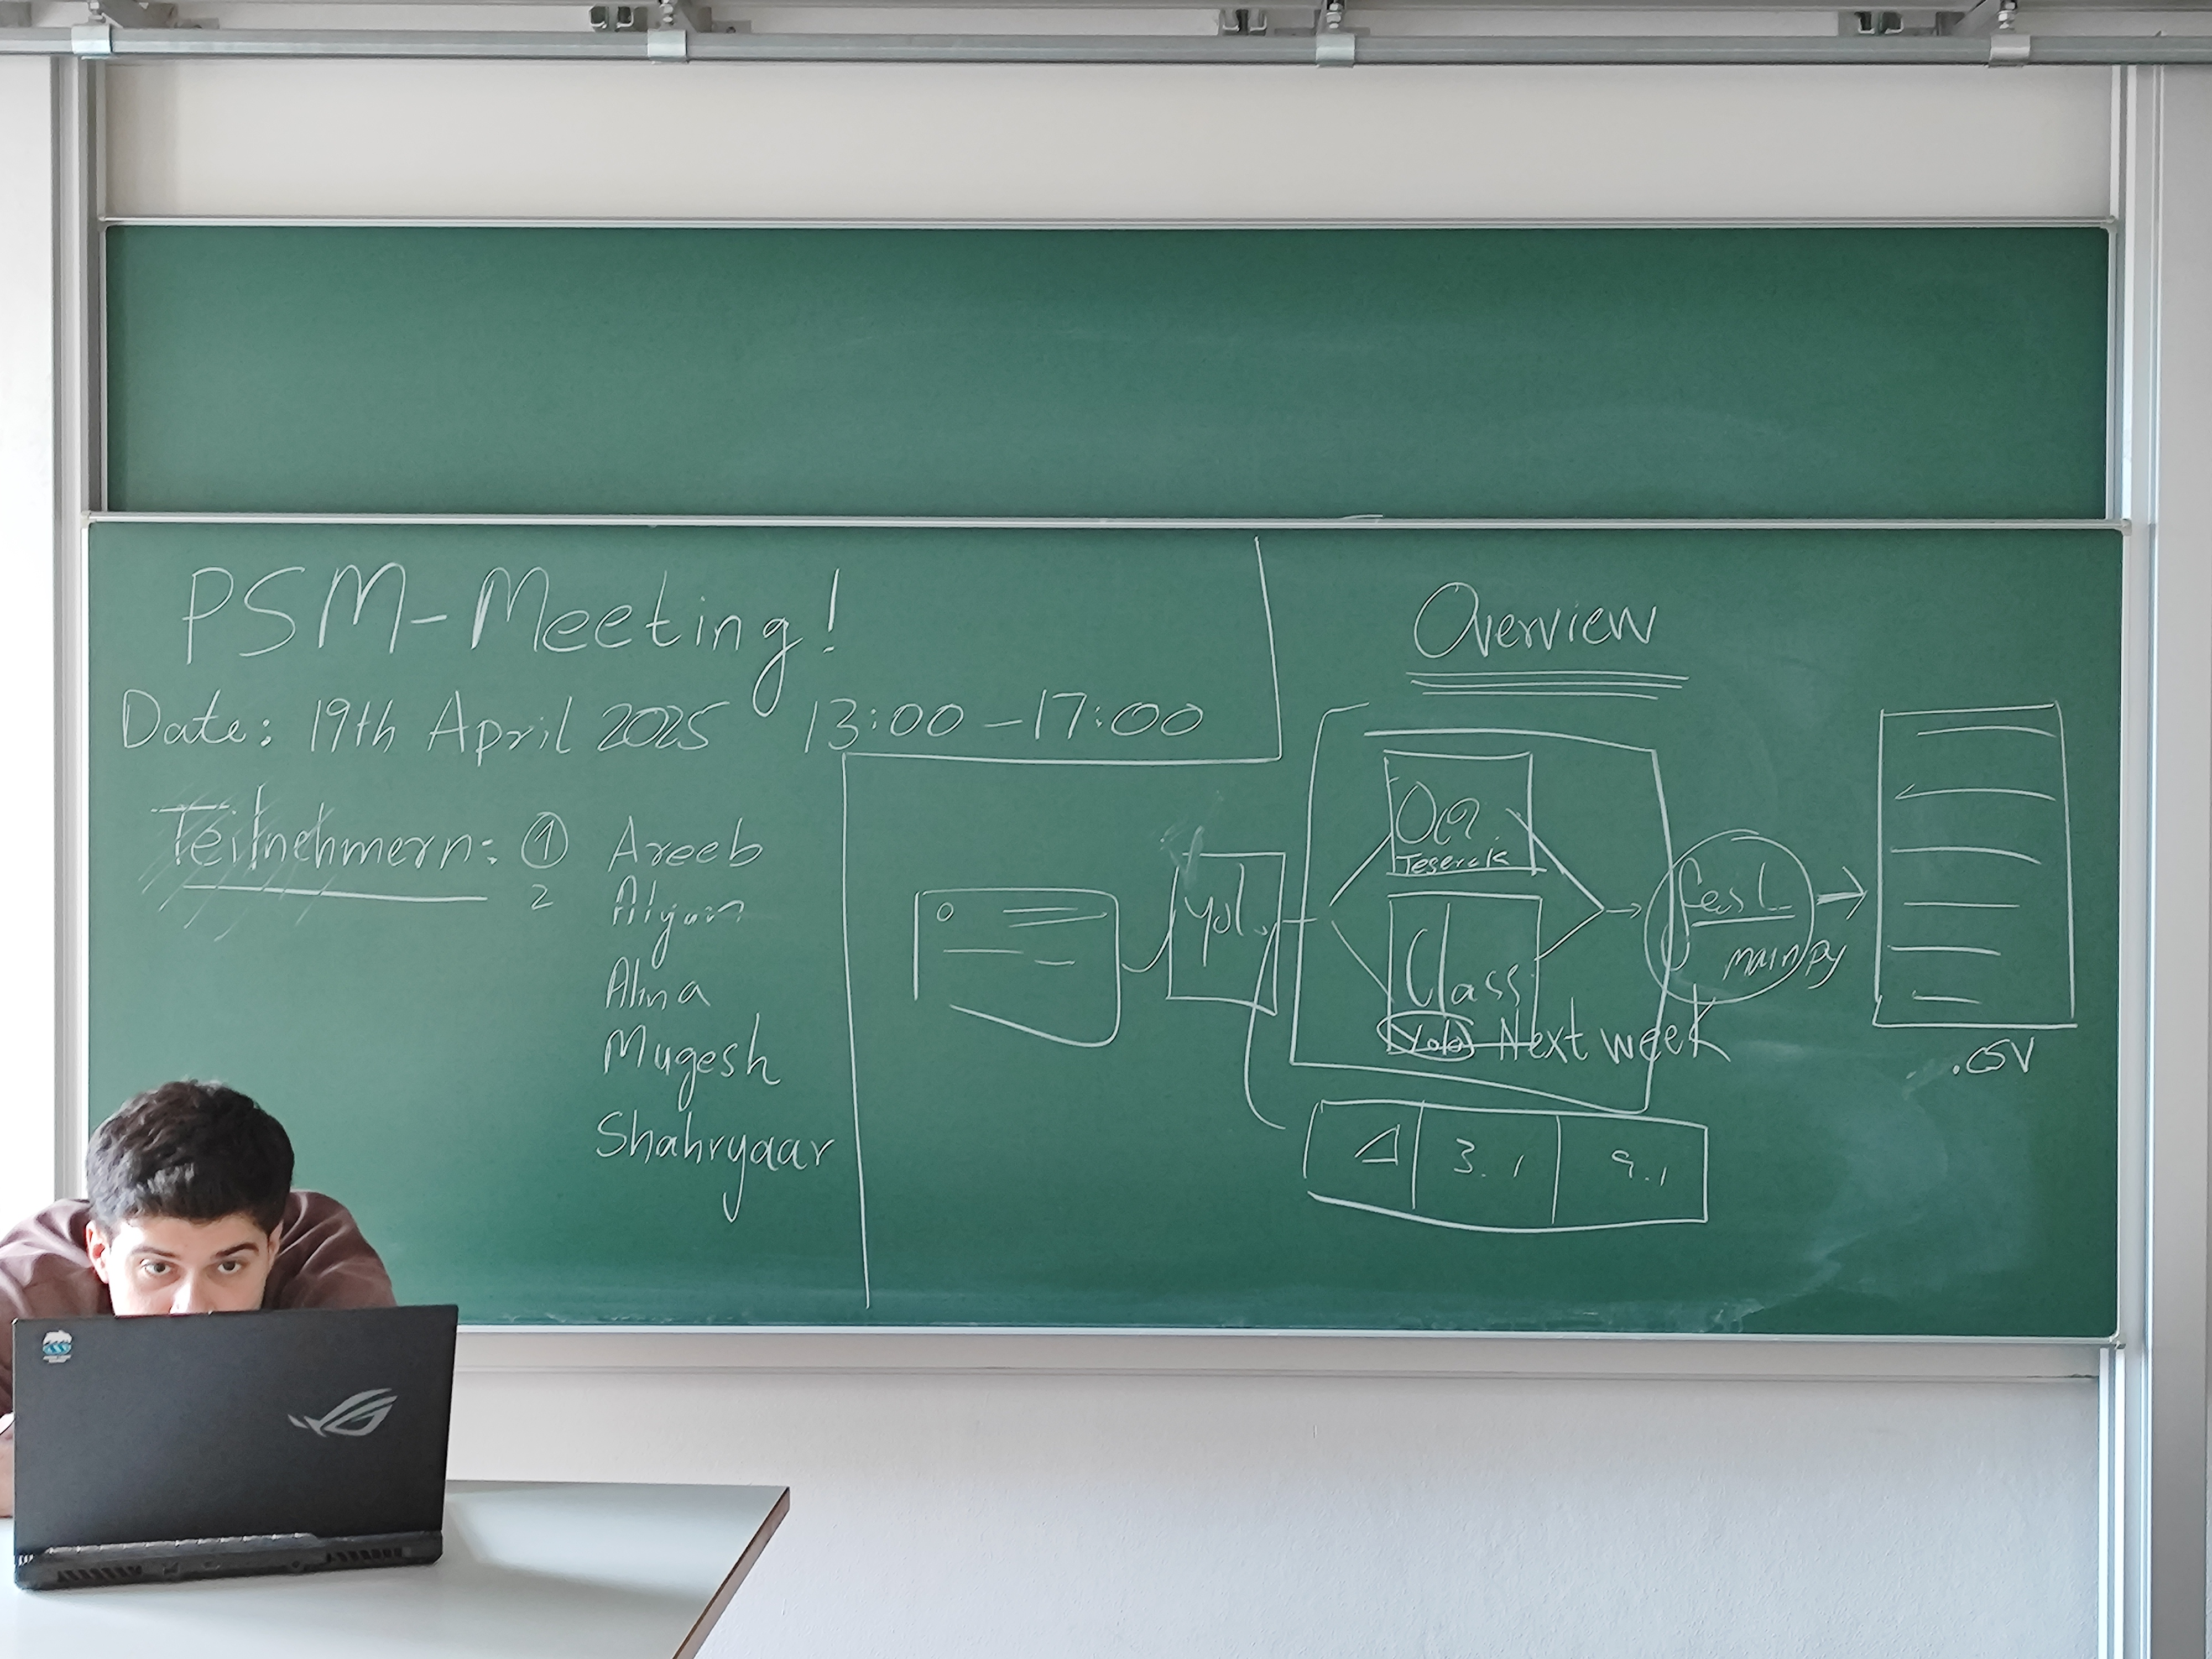
\includegraphics[width=0.8\textwidth]{images/Meeting1.jpg}
    \caption{First offline meeting held on 19th April 2025}
\end{figure}

\section*{Second Meeting (Saturday, 26th April 2025)}

\begin{figure}[H]
    \centering
    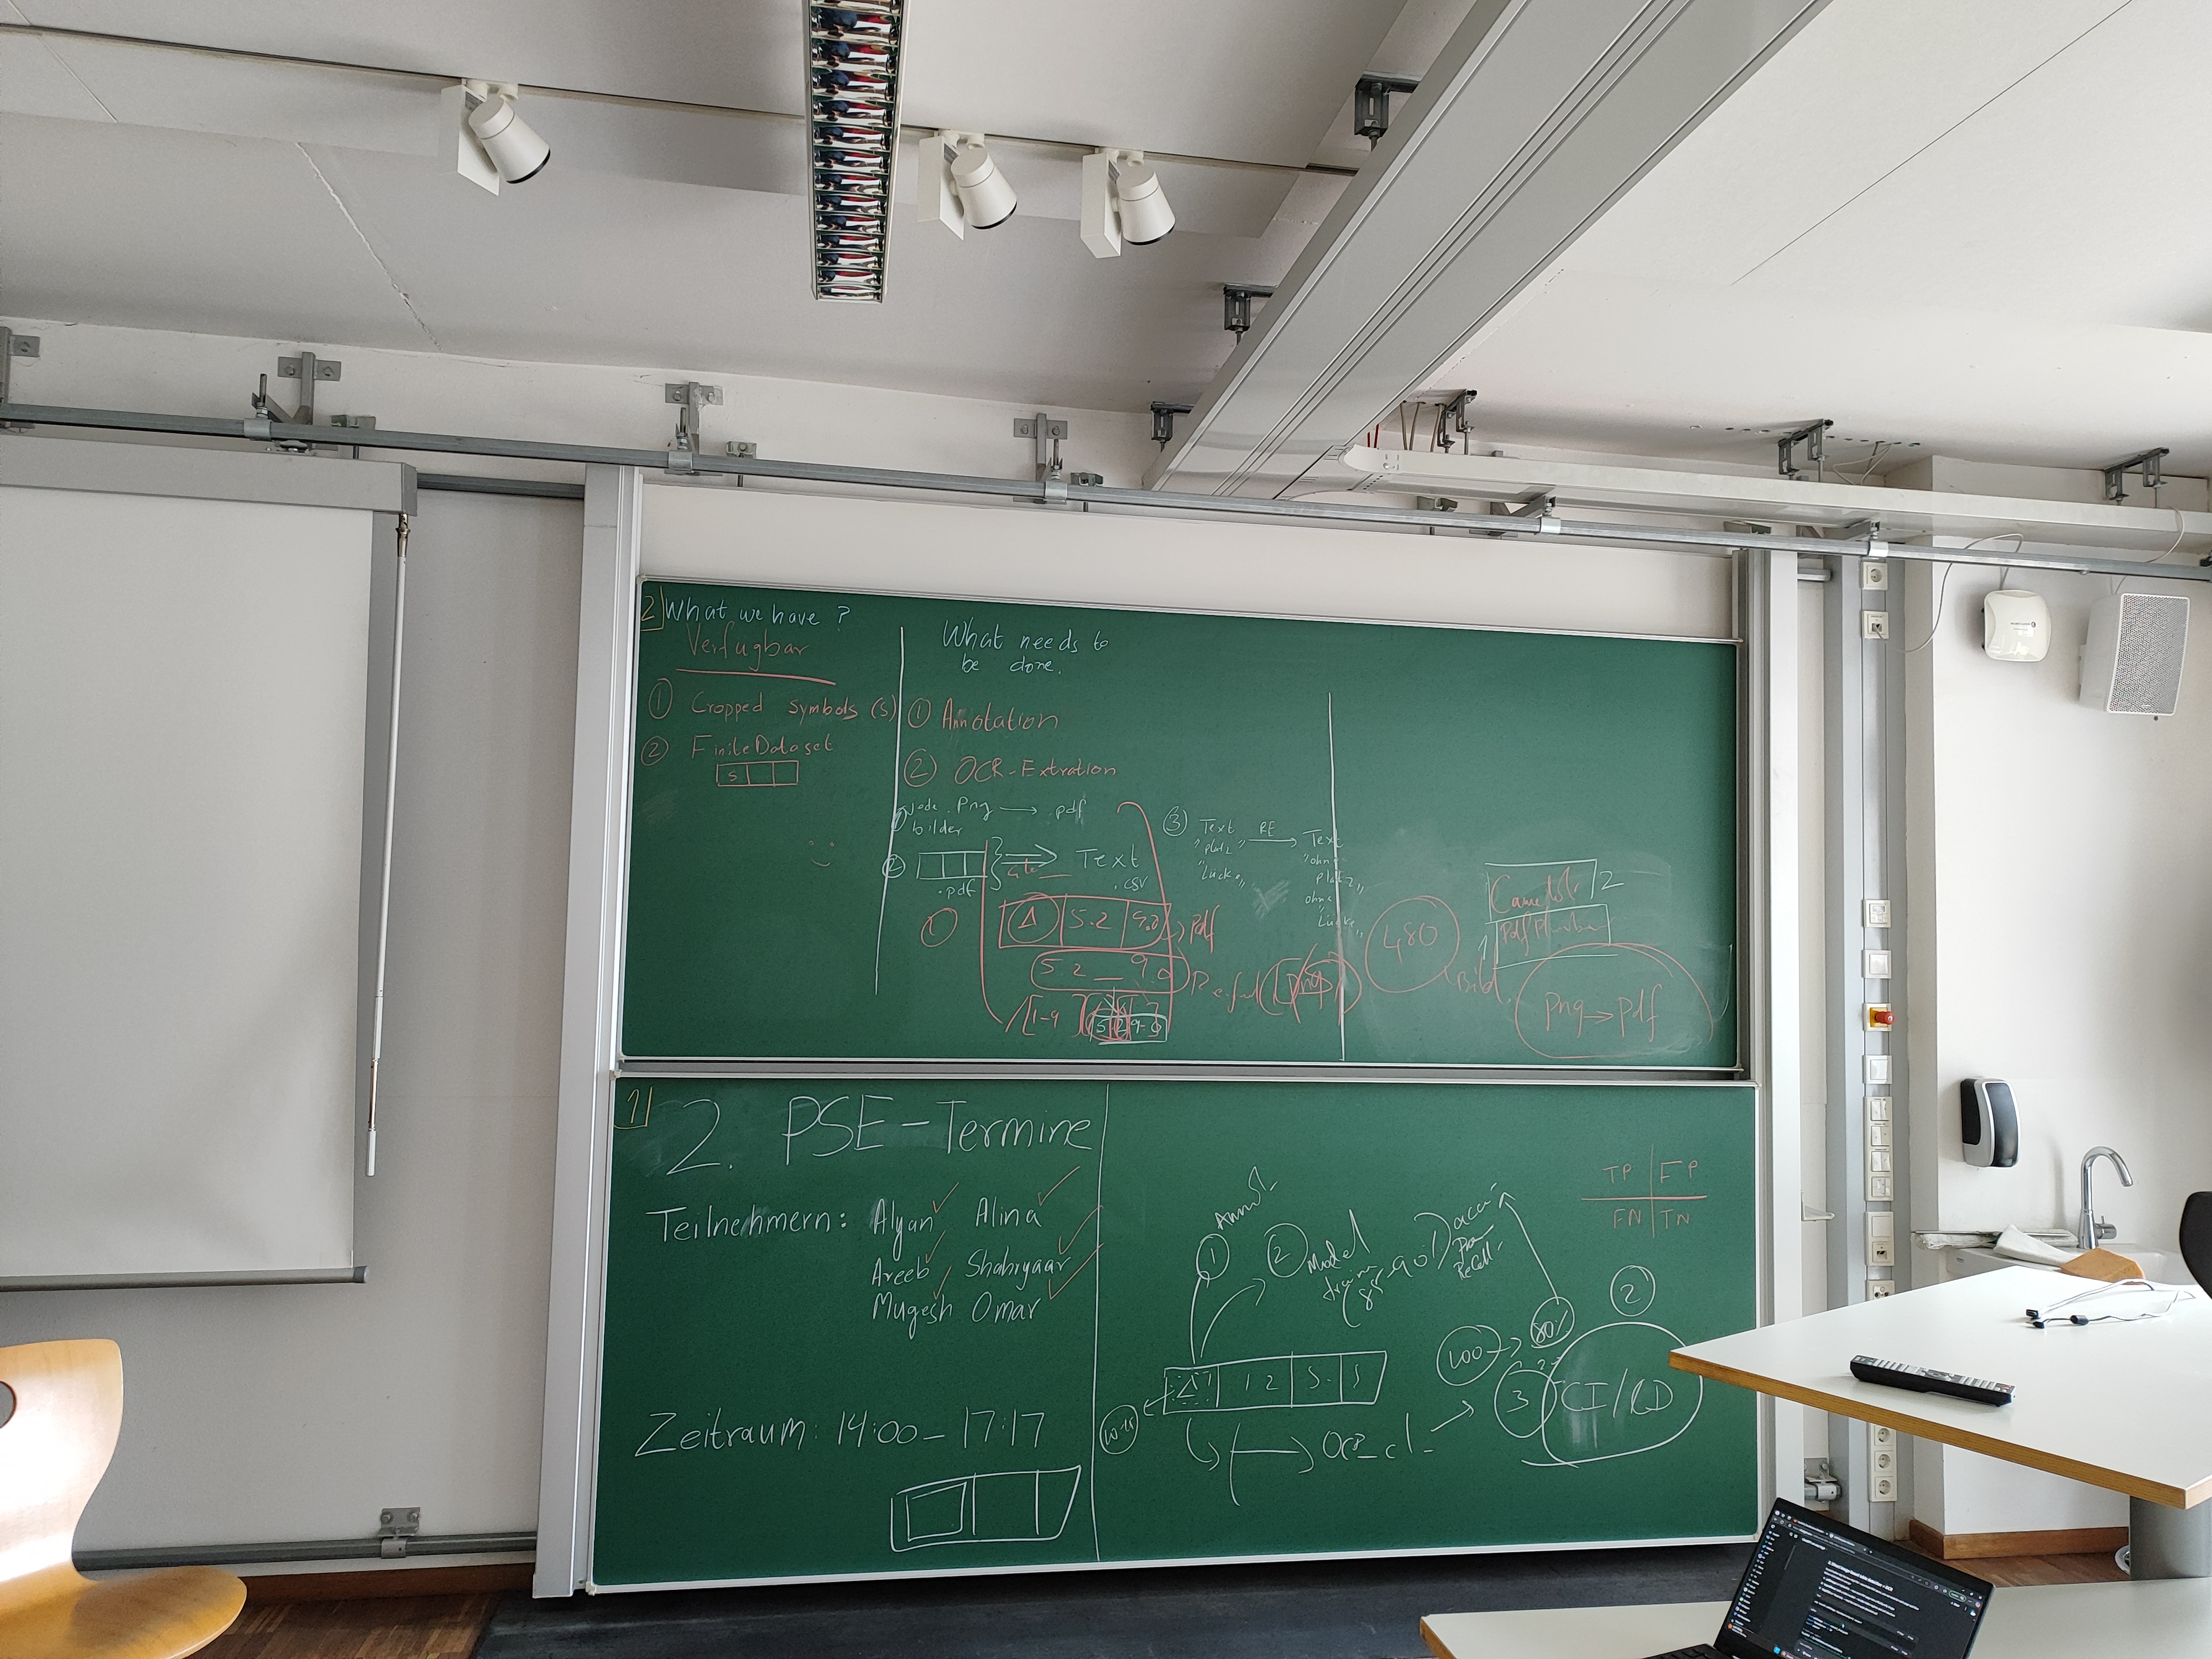
\includegraphics[width=0.8\textwidth]{images/Meeting2.jpg}
    \caption{Second offline meeting held on 26th April 2025}
\end{figure}

\section*{Structure}

\begin{itemize}
    \item Images are stored in the same folder as this document.
    \item Notes or additional documents can be added if necessary.
\end{itemize}

\section*{Purpose}

To keep a record of offline collaboration activities and meeting outcomes for better tracking and transparency.

\end{document}
